~\vspace{.1in}

\section{Modeling with exponential equations}

My grandmother was born in eastern Europe at the end of the 1800s.  When she was eight years old her parents brought her and her younger sister and brother to the United States to escape harsh treatment by the government.  Both her parents had to work, so my grandmother dropped out of school when she was thirteen years old to take care of the children, which now included another brother and sister. 

Time passed and she married a handsome young veteran of World War I, who had also immigrated to the country as a young child.  
For her wedding dowry his parents bought my grandmother a set of sterling silverware, valued at \$800 in 1920.  My grandmother was very proud of her sterling and used it often.

Over the years, the sterling has increased in value, let's say by around 3\% per year.  In 1957, my grandmother handed it down to my mother as a wedding present.  In 1990, I married and my mother handed the sterling down to me.   What was it was it worth at those times, and how much should it be insured for through 2015?  

Let's write the equation to answer these questions.  The variables should be

\begin{tabular} {l} 
$S=$ value of sterling (\$) $\sim$ dep \\ 
$Y =$ time (years since 1920) $\sim$ indep \\
\end{tabular}


We're saying that the sterling increased 3\% per year in value.  For example, in 1921, the sterling was worth
$$\$800 + 3\% \text{ of } \$800 = 800 + .03 \times 800 = 800 + 24= \$824$$
Remember the shortcut here? 
$$800 \times 1.03 = 824$$
The idea is after one year we have the original \$800 plus 3\% more for a grand total of 103\% of what we had before.  And 103\% = 1.03.  

After 5 years, the sterling was worth
$$800 \ast 1.03 \ast 1.03  \ast 1.03  \ast 1.03  \ast 1.03 = 800 \ast 1.03^5$$ 
since multiplying by 1.03 five times is the same as multiplying by $1.03^5$.
On the calculator we do
$$800 \times 1.03 \wedge 5 = 927.4192594 \approx \$927$$

Generalizing, we get our equation $$800 \times 1.03 \wedge Y= S$$
which can be rewritten as $$S=800 \ast 1.03 ^ Y$$
This equation fits our template for an exponential equation
$$\text{dep }=\text{ start } \ast \text{growth factor}^{\text{indep}}$$

Quick recap.  A function is \textbf{exponential} if it corresponds to a fixed percent increase (or decrease).  The percent increase is the \textbf{growth rate}; in our example, the growth rate is  $r=3\%=.03$.  The number we multiply by is the \textbf{growth factor} and it is also the base of the power in the equation; in our example, the growth factor is $g =  1.03$. The \textsc{Percent Change Formula} from Section 2.2 reminds us that $$g=1 + r = 1+.03 =1.03$$

Let's answer those questions.  In 1957, we had $Y = 1957 - 1920 = 37$ years and so $$S = 800\ast1.03^{37} = 800 \times 1.03 \wedge \underline{37}= 2388.18134\ldots \approx \$2,388$$
By 1990, we had $Y = 1990 - 1920 = 70$ years and so $$S = 800\ast1.03^{70} = 800 \times 1.03 \wedge \underline{70}= 6334.2575\ldots \approx \$6,334$$
By 2015, we have $Y = 2015 - 1920 = 95$ years and so $$S = 800\ast1.03^{95} = 800 \times 1.03 \wedge \underline{95}= 13262.5286\ldots \approx \$13,262$$

Let's summarize this information in a table and draw a graph.

\begin{tabular} {|c| |c  |c |c |c |c |c|}\hline
year & 1920 & 1921 & 1925 &  1957 & 1990 & 2015 \\ \hline
$Y$ & 0 & 1 & 5 & 37 & 70 & 95 \\ \hline
$S$ & 800 & 824 & 927 & 2,388 &  6,334  &  13,262 \\ \hline
\end{tabular}


\scalebox {.9} {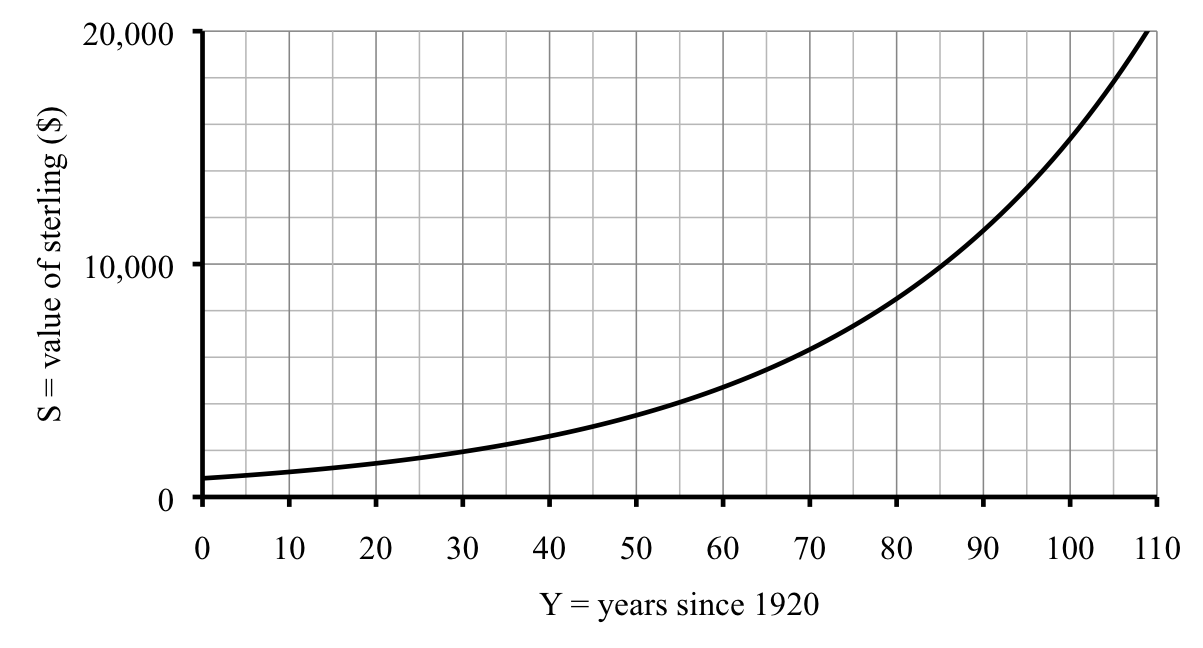
\includegraphics [width = 6in] {grandmasterling.png}}


Actually, the insurance policy allows for up to \$20,000. The curve we drew suggests that the value will be \$20,000 just past $Y=100$ (the year 2020), probably somewhere around $Y=110$ (the year 2030).  

We can use successive approximation to improve our answer. 

\begin{tabular} {|c| |c  |c |c |c|}\hline
year & 2020 & 2030 & 2029 &  2028  \\ \hline
$Y$ & 100 & 110 & 109 & 108\\ \hline
$S$ & 15,375 & 20,663 & 20,061 & 19,476\\ \hline
vs.\ 20,000& low & high & high & low \\ \hline
\end{tabular}

Seems to around the year 2029, where $Y=109$, as we had guessed.

Of course, we can solve the exponential equation instead. To find when $S= 20,000$ we use our equation $S = 800 \ast 1.03^Y$ to get 
$$800 \ast 1.03^Y =  20,000 $$
Divide each side by 800 to get
$$ \frac{\cancel{800} \ast 1.03^Y}{\cancel{800}} = \frac{ 20,000}{800} $$
and so $$1.03^Y = \frac{ 20,000}{800}  =  20,000 \div {800} = 25$$
Since we want to solve for the exponent, we use the \textsc{Log-Divides Formula} with growth factor $g=1.03$ and the value $v= 25$ to get
$$Y =  \frac{\log (v)}{\log(g)} =  \frac{\log (25)}{\log(1.03)} = \log (25) \div \log (1.03) = 108.89737 \approx 109  $$
We rounded up to make sure it would reach the full \$20,000.  Since 1920 + 109 = 2029, we see (again) that the value should reach \$20,000 in the year 2029.

As an aside, look what happens when we calculate the rate of change for this function.  For example, during the first five years, 
$$\text{rate of change} =  \frac{\text{change dep}}{\text{change indep}} = \frac{\text{\$927} - \text{\$800}}{1925-1920}= \frac{\$127}{5 \text{ years}} = 127 \div 5 = \$25.40\text{/year}$$
and from 1925 to 1957, 
$$\text{rate of change} =  \frac{\text{change dep}}{\text{change indep}} = \frac{\text{\$2,388} - \text{\$927}}{1957-1925}= \frac{\$1,461}{32 \text{ years}} = 1,461 \div 32 \approx \$45.66\text{/year}$$
In the first few years, the value increased an average of \$25.40 a year, but from 1925 to 1957 it increased an average of about \$45.66 per year.

Were we supposed to get different numbers here?  Well, the graph's not a line and it's not a linear equation.  That tells us the rate of change isn't going to be constant.  So, sure, different numbers are fine.  Does it make sense that the rate of change would itself increase?  That the value increases at an increasing rate? Yes. Although we are always just adding on 3\%, we're taking 3\% of larger numbers each year.  So more is added each year.  

 %\section{Modeling with exponential equations}

 \begin{center}
\line(1,0){300} %\line(1,0){250}
\end{center}

\section*{Homework}

\noindent \textbf{Start by doing Practice exercises \#1-4 in the workbook.}

\bigskip
 
\noindent \textbf{Do you know \ldots}

\begin{itemize} 
\item What makes a function exponential? 
\item The template for an exponential equation? \emph{Ask your instructor if you need to remember the template or if it will be provided during the exam.} 
\item How to write an exponential equation given the starting amount and percent increase?     
\item Where the growth factor and starting amount appear in the template of an exponential equation?  
\item What the graph of an exponential function looks like?  
\item How to solve an exponential equation using the \textsc{Log Divides Formula}?   

\emph{Ask your instructor if you need to remember the \textsc{Log Divides Formula} or if it will be provided during the exam.}  
\item How to calculate the rate of change of an exponential function?     
\item Why the rate of change of an exponential function is not constant?     
\end{itemize}

\subsection*{Exercises}

\begin{enumerate} 
\setcounter{enumi}{4}

\item Use the equation from this section for the value of the sterling silverware to determine when the sterling was first worth over \$\text{5,000}.
\begin{enumerate}
\item First, estimate the answer from our table and graph.
\item Next, use successive approximation to refine your answer. Display your work in a table.
\item Last, practice setting up and solving an equation using the \textsc{Log Divides Formula}.
\end{enumerate}

\item Mrs.\ Nystrom's Social Security benefit was \$746.17/month when she retired from teaching in 2009. She had taught in elementary school since I was a girl.   Benefits have increased by 4\% per year.   \hfill \emph{Story also appears in 1.1 and 1.2  Exercises} 
\begin{enumerate}
\item Name the variables and write an equation relating them.
\item Use your equation to estimate her benefit in the year 2020.
\item Set up and solve an equation to determine when her benefit will pass \$900/month.
\item Repeat for \$\text{1,000}/month.
\end{enumerate}  

\item The number of players of a wildly popular mobile app drawing game  has been growing exponentially according to the equation $$N = 2 \ast 1.57^W$$ where $N$ is the number of players (in millions) and $W$ is the number of weeks since it caught on.
\hfill \emph{Story also appears in 5.1 \#3 and 5.3 Exercises}
 % Source: Wikipedia (Draw Something) 5 weeks 20 million, 50 days 50 million
\begin{enumerate}
\item Make a table showing the number of players after 0 weeks, 2 weeks, 4 weeks, and 6 weeks.  
\item Use successive approximation to determine when there will be over 60 million players.  Round your answer to the nearest week.
\item Show how to solve the equation to determine when there will be over 60 million players.  Record your answer to two decimal places.  
\item Use your answer to (a), (b), and (c) to graph the function.
\end{enumerate} 

\item In 2006 there were about 5.2 million people living in the state of Minnesota.  Predicted growth rates vary, perhaps around .5\% per year. % SU in 2010 it was 5.3  % Source MN dept of administration
\begin{enumerate}
\item What is the annual growth factor?  Careful, the growth rate is .5\%
\item Based on these figures, about how many people will be living in the state of Minnesota in 2010?  In 2020?  
\item Write an equation showing how Minnesota's population is a function of the year.  Don't forget to name the variables.
\item Make a table of values showing the projected population every two years from 2006 to 2020.  
\item Draw a graph illustrating the dependence.
\item Set up and solve an equation to determine when Minnesota's population is expected to be double the population from 2006.
\end{enumerate}

\item Um Archivo data consultant group reported earnings of \$42.7 billion in 2012.  At that time executives projected 17\% increase in earnings annually.  Based on that information, we wrote the equation $$U = 42.7 \ast 1.17^Y$$ where $U$ is Um Archivo's reported earnings (in \$billions) and $Y$ is the years since 2012.
\hfill \emph{Story also appears in 2.2 Exercises}
\begin{enumerate}
\item According to your equation, in what year would Um Archivo's reported earnings pass \$60 billion?  Set up and solve an equation.  Then check your answer.
\item Repeat for \$100 billion.
\end{enumerate}  

\item In 1990 it was estimated that 2.5 million households watched reality television at least once a week.  Executives predicted that number would increase by 7.2\% each year.  According to their estimates, how many millions of households watched reality television in 2000?  In 2010?  As part of your work, name the variables, find the annual growth factor, and write an exponential equation modeling reality television viewing.

\hfill \emph{Story also appears in 5.2 \#3}

\end{enumerate}




